\newpage
\section{Design and Implementation}
    \subsection{Input format}
    The input is the \textbf{Bayesian Interchange Format} (BIF) which is a file with .bif extension.
    In general, Four types of blocks are defined.\\
    \noindent \textbf{The Network Block:}\\
    A network block defines the name of the network and lists the properties. The example below specify the network block for the Asia Bayesian Network:
    \begin{lstlisting}
    network asia{
       property version 1.1;
       property author ..;
    }
    \end{lstlisting}
    
    \noindent \textbf{The Varable Block:}\\
    Variable blocks define the variables in a network. These blocks used
    to be called node blocks in the BNIF; it seems that variable conveys
    more of a statistical meaning while node just refers to a graphical
    concept. The example below is the bronc node from asia.bif
    \begin{lstlisting}
     variable bronc{
        type discrete [2] {yes, no};
     }
    \end{lstlisting}
    
    \noindent \textbf{Blocks for standard nodes}\\
    Standard nodes have to define the probabilities for each discrete parent instantiation. An example of a standard probability block is: 
    \begin{lstlisting}
     probability (dysp | bronc, either){
        (yes, yes) 0.9, 0.1;
        (no, yes) 0.7, 0.3;
        (yes, no) 0.8, 0.2;
        (no, no) 0.1, 0.9;
    }
    \end{lstlisting}
    
    \noindent \textbf{Probability blocks}:\\
    Probability blocks are another way to specify the (conditional) probability tables (CPTs). For these variables, and hence the topology of the network. The block indicates the variables of the probability distribution right after the keyword probability.
    \begin{lstlisting}
    probability (v_10_8 v_10_7 v_9_8){ 
	table 0.586357 0.667473 0.789088 0.466932 
	      0.413643 0.332527 0.210912 0.533068;
    }
    \end{lstlisting}
    A more detailed explanation of the BIF is explained here: \footnote{http://www.cs.washington.edu/dm/vfml/appendixes/bif.htm} \\
    
    \subsection{Output}
    The output of the program is the cnf file following the DIMACS format which is a widely accepted standard format for representing CNF clauses and it's also a format used by most of the model counters mentioned in section 3.3.\\
    \begin{itemize}
        \item A comment line starts with a \textit{c}
        \item A line p cnf var clauses specify the instance in CNF format, in which \textit{vars} is the number of variables used in the file and \textit{clauses} is the number of clauses in the CNF.
        \item Each CNF variable is denoted by a non\-zero number smaller than \textit{vars}, the negation of a variable is denoted by a negative number.
        \item Each clauses contains one or several CNF variables, 0 specifies the end of the clause.
    \end{itemize}
    
    Consider the following CNF:
    \begin{center}
        $x_{1} \vee x_{2} \vee \neg x_{3}$\\
        $x_{1} \vee x_{4} \vee x_{5}$\\
        $\neg x_{3} \vee \neg x_{4}$\\  
    \end{center}
    The clauses in DIMACS format:
    \begin{center}
        \begin{lstlisting}
        c A sample DIMAC file
        p cnf 5 3
        1 2 -3 0
        1 4 5 0
        -3 -4 0
        \end{lstlisting}
    \end{center}
    
    \subsection{Extend the pgmpy library}
    Pgmpy library does not support fetching CPT values using table indexing, the only way to fetch value is through specifying evidence and variables and query the value through Variable Elimination method. The Variable Elimination method is the bayesian inference method that is \textcolor{red}{Insert time complexety}. To solve the problem, I extended the pgmpy library to support fetching variable values without querying using Variable Elimination.\\

    \textbf{The TabularCPD Class}:\\
    The method get\_cpds returns a conditional probability distribution of the node, the returned type is defined as TabularCPD that contains the name of the node, cardinality, variables which are stores as a nested list, the list of evidences and their corresponding cardinalities. An example is given below:
    \begin{lstlisting}
    cpd = TabularCPD('dysp', 2, [[0.9, 0.7, 0.8, 0.1],
                                 [0.1, 0.3, 0.2, 0.9]],
                                 ['bronc', 'either'], [2, 2])
    \end{lstlisting}

    \textbf{The storage of a TabularCPD}:\\
    calling cpd.variables() will return a list starts with the node variable followed by the the evidences, and calling cpd.cardinality() will return the cardinality list in the same order as the variables returned by cpd.variables()
    \begin{lstlisting}
    >> print(cpd.variables())
        >> ['dysp', 'bronc', 'either']
    >> print(cpd.cardinality())
        >> ['2', '2', '2']
    \end{lstlisting}

    \textbf{MyCPD}:\\
    col\_index stores the index of the combination of evidence, in the same order as the probability distribution defined in the \textbf{standard node block}. The col\_index is constructed using the itertools.product in python which return the cartesian product. The transpose of the col\_index correspond to the order of the probability distribution specify in the BIF file. Consider the example with node \textit{dysp}.
    \begin{lstlisting}
    >> col_indexes = np.array(list(product(*[range(i) for i in ev_card])))
    >> print(evidence, col_index) 
        >> ['either', 'bronc']
        >> [[0 0]
            [0 1]
            [1 0]
            [1 1]]
    \end{lstlisting}
    \textcolor{red}{Maybe I should save some space}.\\
    Then the evidences are formatted into tuples with the same length and each column correspond to one entrance to the probability table.\\
    \begin{lstlisting}
    A sample return the evidence entrance. 'dysp' node in aisa.bif
    >> entrance <- [('{s}'.format(s = reverse_ev[i]), d) 
                    for d in col_indexes.T[i]]
        >> [('either',0), ('either',0), ('either',1), ('either',1)]
           [('bronc', 0), ('bronc', 1), ('bronc', 0), ('bronc', 1)]
    Then the entrace are transposed using rol_to_col()
    >> rol_to_col(entrance)
        >> [[('bronc',0), ('either',0)], [('bronc',1), ('either',0)], 
            [('bronc',0), ('either',1)], [('bronc',1), ('either',1)]]
    \end{lstlisting}
    
    \begin{minted}
    [linenos]
    {python}
    Parameter: A TabularCPD
    def myCPD(TabularCPD cpd):
        var, evidence <- cpd.variable[0], cpd.variable[1:]
        var_card, ev_card <- cpd.cardinality[0], cpd.cardinality[1:]
        variable <- [(name, 0),.., (name, n)]
        value = cpd.values()
        # node with evidence:
        if evidence not null:
            col_indexes <- get index
            for i in cardinality:
                entrance <- format the header
                rol_to_col(entrance) # transpose
            for each node variable:
                newcpt.append(variable, index, evidence, corresponding_value)
        # node with no evidence
        else:
            for each node variable
                newcpt.apend(variable, index, [], corresponding_value)
    \end{minted}
    A Sample return of newcpt of node dysp:
    \begin{lstlisting}
    [('dysp', 0, [('bronc', 0), ('either', 0)], 0.9), 
     ('dysp', 0, [('bronc', 1), ('either', 0)], 0.7), 
     ...
     ('dysp', 1, [('bronc', 0), ('either', 1)], 0.2), 
     ('dysp', 1, [('bronc', 1), ('either', 1)], 0.9)]
    \end{lstlisting}
    The method mycpd(TabularCPD) returns a table\-like list of tuples, the first two element in each tuple forms the node variables and the third element is a list of evidence. An example of the first tuple in the list means $dysp_{0}|bronc_{0}either_{0} = 0.9$. Now the returned data support fetching values using list indexing so that we don't need to query the value using the time-consuming Variable Elimination.\\ 
    
    
    In our case for both bronc and either, the evidence all equals to 2, the convention for the order is shown in figure \ref{fig:sample print table}. The list which store the values are the transpose of the matrix in BIF format.\\
    \begin{figure}
        \centering
        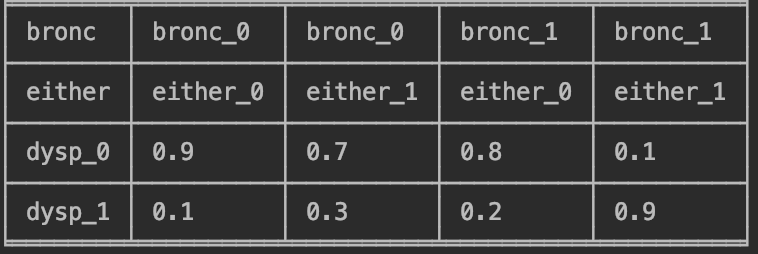
\includegraphics[width = 0.7\textwidth]{pic/printBayesnode.png}
        \caption{A sample printed CPT of a node dyps}
        \label{fig:sample print table}
    \end{figure}
    \subsection{Implementation of Full encoding}
    In section 3.1 Full encoding, for each node in the Bayesian network, two kinds of variables need to be generated, indicator variables and parameter variables respectively. This section will first show the steps to generate indicator variables and indicator clauses and then show the steps to encode parameter variables and clauses.
    \begin{itemize}
        \item \textit{var\_dic} is a dictionary in which the key is the name of the variable and the value is used when the cnf is written into the DIMACS format. 
        \item \textit{clauses} is a nested list, each element correspond to one clauses in the generated CNF. Literals are stores as a tuple (sign, variable). sign = -1 means the negation of the variable
        \item \textit{weights} is a dictionary that stores the corresponding weights of the variable following the weights assigning rules mentioned in \textcolor{red}{WHICH SECTION}. The key is the name of the variable such as $\lambda_{dysp_{0}}$ and the value is the corresponding weight.
    \end{itemize}
    \textbf{Generating Indicator variables:}\\
    Given a bayesian network \textit{bn}, for each node in the network, define the number of indicators same as its cardinality. Then two types of clauses are generated: $[\lambda_{x_{1}}, ... \lambda_{x_{n}}]$ and $[\neg \lambda_{x_{i}}, \neg \lambda_{x_{j}}]$ when $i < j$. weights($\lambda_{x}$) = 1, weights($\neg \lambda_{x}$) = -1. Traverse the node in the given Bayesian network and all indicator clauses are generated.
    The Psuedocode for generating indicator variables and clauses is given below:
    \begin{minted}
    [linenos]
    {python}
    def indicator(bn, var_dic, clauses, weights):
        for i in bn.nodes:
            cardinality <- bn.get_cardinality(i)
            # get variables
            for j in range(cardinality):
                name <- 'lambda_' + str(i)+ '_' + str(j)
                # append variable to variable dictionary
                # store the corresponding weights
                if name not in var_dic:
                    var_dic[name] = max(var_dic.values()) + 1
                    weights[name] = 1
            # get clauses:
        for i in bn.nodes:
            cardinality <- bn.get_cardinality(i)
            cl = [] # cl store each clause in the CNF, represented by a list of tuples
            for j in range(cardinality):
                variable <- fetch the corresponding variable from the dictionary
                cl.append((1, variable)) # 1 represent positive
            clauses.append(cl)
            
            for m in range(cardinality):
                for n in range(m + 1, cardinality):
                    var1, var2 <- fetch lambda_i_n, fetch lambda_i_m
                    cl = [(-1, var1), (-1, var, var2)]
                    clauses.append(cl)
                    weights[m] = -1
    return clauses, var_dic, weights
    \end{minted}
    
    \noindent \textbf{Generating Parameter variables:}\\
    For each variable of a node in the bayesian network, first get the evidence of the variable and the the evidences' cardinality. These, together with the node's cardinality, specify the number of values in a conditional probability table. For each value, a parameter variable $\theta_{node_{i}|evidences}$ is generated.\\
    $$number\_of\_values = cardinality(node) \times \Pi_{i = 1}^n cardinality(evidence_{i})$$
    
    The corresponding clauses: (described in line 20 \~ 26 in psuedocode)
    \begin{itemize}
        \item $ \neg\lambda_{x_{i}} \vee \neg\lambda_{y_{1}} \vee... \vee \neg\lambda_{y_{m}} \vee \theta_{x_{i}|y_{1}..y_{m}}$
        \item  $\neg\theta_{x_{i}|y_{1}..y_{m}} \vee \lambda_{x_{i}}$
        \item $\neg\theta_{x_{i}|y_{1}..y_{m}} \vee \lambda_{y_{j}} \;\; \mbox{ j = 1, ..., m}$
    \end{itemize}
    
    \begin{minted}
    [linenos]
    {python}
    def parameter_cl(bn, var_dic, clauses, weights):
        for i in bn.nodes:
            cardinality = i.get_cardinality()
            evidence = i.get_evidence()
            if no evidence:
                for j in cardinality:
                    name <- theta_ij
                    var_dic[name] <- max(var_dic.value()) + 1
                    weight[name] <- fetch weight
                    clauses.append([(-1, var_dic['lambda_i']), (1, var_dic[name]])
                    clauses.append([(-1, var_dic[name]), (1, dic['lambda_i'])])
            else:
                ev_cardinality <- [ev.cardinality() for ev in i.evidence]
                evidence_lst <- generate evidence list()
                for j in cardinality:
                    for ev in evidence_lst:
                        name = 'theta_' + i + str(j) + '|' + ev
                        var_dic[name] <- max(var_dic.value()) + 1
                        weight[name] <- fetch weight
                        clauses.append([(-1, var_dic['lambda_i']),
                                        ...
                                        (-1, var_dic['lambda_evidences']),
                                        (1, var_dic[name]])
                    clauses.append([(-1, var_dic[name]), (1, dic['lambda_i'])])
                    ...
                    clauses.append([(-1, var_dic[name]), (1, dic['lambda_evs])])
    return var_dic, clauses, weights
    % \caption{Psuedocode for encoding parameter clauses}
    % \label{code:Full enc parameter clauses}
    \end{minted}

    \subsection{Simplified Full encoding}
    In simplified Full encoding, one of the main improvement is to capture the extreme values when generating the parameter clauses. Before generating variables and clauses, the weight is fetched from the Probabilty table.\\
    \newline
    If Pr($variable_{i}|evidence_{1}...evidence-{m}$) = 0, the parameter clauses won't be generated, and only one clause will be appended to the CNF: [$\neg \lambda_{variable_{i}|}, \neg \lambda_{evidence_{1}}, ..., \neg \lambda_{evidence_{m}}$].\par
    If Pr($variable_{i}|evidence_{1}...evidence-{m}$) = 1, no action is done and the program should move to the next entry of the probability table.\\
    
    The psuedocode for simplifying extreme values with evidence list not empty is given below, the case without evidence can be implemented similarly.
    \begin{minted}
    [linenos]
    {python}
    for i in bn.nodes:
        for j in i.get_cardinality():
            evidence = i.get_evidence()
            # case with evidence:
            if evidence not null:
                parameter_value <- fetched weight
                if parameter_value == 0:
                    clauses.append([(-1, var_dic[lambda_ij]),
                                    (-1, var_dic[lambda_evidence1]), 
                                    ... ,
                                    (-1, var_dic[evidence_m])])
                if parameter_value == 1:
                    continue
                else: 
                    do the same as Full encode parameter clauses
        
    \end{minted}
    According to \textcolor{red}{PAPER NAME}, the simplification step lead to significant improvement in the number of clauses which directly influence the time and space usage in the model counting phase. Detailed result is discussed later in the Result section \textcolor{red}{result section number}
    
    \subsection{Implementation of Improved Encoding}
    The idea of Improved encoding is to use same logic variable to encode the parameter variables that have the same value in the CPT. For each node in the Bayesian network, the table is first partitioned in to several sub-tables based on the probability values. This can be done with the sorting within the table fetched by myCPD(TabularCPD) method.
    \subsubsection{Splitting the CPT}
    
    \subsubsection{Encoding each parameter value}
    
    \subsection{Implementation of Group Encoding}
        
    \subsubsection{QM algorithm and extension for multi-variate simplification}
    
    \subsection{Write files}
  
